\documentclass[a4paper,fleqn]{cas-sc}

\usepackage[authoryear]{natbib}
\usepackage{graphicx}
\usepackage{float}
\usepackage{color}
\usepackage{setspace}
\usepackage{booktabs}
\usepackage{array}
\usepackage{multirow}
\usepackage{amsmath,amssymb,amsfonts}
\usepackage{enumitem}
\usepackage{xcolor}
\usepackage{url}
\usepackage{lineno}

\begin{document}
\let\WriteBookmarks\relax
\def\floatpagepagefraction{1}
\def\textpagefraction{.001}
\shorttitle{Reproducible DINOv2 Workflow for Low-Shot RSSC}
\shortauthors{Hou}

\title[mode = title]{A Reproducible DINOv2 Workflow for Low-Shot Remote Sensing Classification}

\author[1]{Chao Hou}
\credit{Conceptualization, methodology, software, validation, visualization, writing - original draft.}

\address[1]{School of Cybersecurity, Xi'an Polytechnic University, Xi'an, Shaanxi, China}

\begin{abstract}
Scarce labels remain a practical bottleneck in geospatial image analysis, yet many remote sensing scene classification studies still rely on protocol-specific settings that are hard to reproduce or compare fairly. Rather than introducing another remote-sensing-specific architecture, we present a reproducible adaptive-transfer workflow for scarce-label scene classification built on \textbf{DINOv2-Base}, fixed class-balanced split manifests, and scripted multi-seed evaluation. The model freezes most pretrained parameters, selectively unfreezes only the last transformer block and final normalization, inserts a residual feature adapter, and applies momentum-updated feature-center regularization. Experiments on AID and NWPU-RESISC45 follow a fixed protocol with 20 training images and 10 validation images per class, and all main comparisons are reported as three-seed averages regenerated from the same experiment outputs. Against a matched-split ConvNeXt-Tiny reference under identical data partitions, the workflow improves mean overall accuracy from 0.9179 to 0.9413 on AID and yields a smaller but still positive increase from 0.8721 to 0.8790 on NWPU-RESISC45. Same-backbone ablations show that selective finetuning provides most of the mean gain, while the adapter mainly reduces seed variance and the feature-center term improves mean performance on both datasets. Although the full backbone is not lightweight in total inference cost, only about 7.5 million parameters are trainable and the final setup remains feasible on an 8 GB GPU. The resulting contribution is a practical geocomputing workflow centered on public data, fixed manifests, and rebuildable evidence rather than on architectural novelty alone.
\end{abstract}

\begin{coverletter}
\raggedright
Dear Editors,

Please consider our manuscript ``A Reproducible DINOv2 Workflow for Low-Shot Remote Sensing Classification'' for publication in Computers \& Geosciences.

This manuscript addresses a practical geocomputing problem: scarce-label remote sensing scene classification under public-data, fixed-protocol evaluation. Rather than proposing another scene-classification architecture, we contribute a reproducible geocomputing workflow that couples DINOv2-Base selective adaptation with persistent split manifests, scriptable multi-seed aggregation, and manuscript-rebuild assets.

We believe the work fits Computers \& Geosciences for three reasons. First, it targets geospatial image analysis on public remote sensing benchmarks under an explicitly documented protocol. Second, its central contribution is a reusable and auditable computational workflow rather than architecture-only benchmarking. Third, the code, configuration, manifests, and reproduction assets are publicly available under the MIT License, with a reviewer-safe archive retained for inspection convenience.

Under one fixed class-balanced protocol, the workflow improves mean overall accuracy on AID from 0.9179 to 0.9413 and yields a smaller positive shift on NWPU-RESISC45 from 0.8721 to 0.8790. We present these results as matched-protocol workflow evidence rather than as universal performance claims. Same-backbone ablations show that selective finetuning provides the primary gain, while the adapter mainly improves stability and the feature-center regularizer improves mean performance under the current protocol.

To support editorial and reviewer inspection, we provide a public repository and a reviewer-safe code packet containing split manifests, experiment scripts, configurations, source modules, generated manuscript tables, and reproduction notes. The manuscript's Code availability section points directly to the live repository.

This manuscript has not been published previously and is not under consideration elsewhere. The author has approved the manuscript and agrees with its submission to Computers \& Geosciences.

Sincerely,\\
Chao Hou\\
School of Cybersecurity, Xi'an Polytechnic University\\
2446099877@qq.com
\end{coverletter}

\begin{highlights}
\item Fixed public split manifests and scripted multi-seed aggregation support reproducible low-shot remote sensing evaluation.
\item The workflow yields a substantial AID improvement and stable cross-benchmark evidence under identical seed-controlled splits.
\item Partial finetuning is the main gain source under the evaluated scarce-label protocol.
\item The workflow package includes rebuildable tables, figures, manifests, and auditable experiment records.
\item Final training remains feasible on a single 8 GB GPU with only about 7.5M trainable parameters.
\end{highlights}

\begin{keywords}
remote sensing scene classification \sep scarce-label learning \sep reproducibility \sep DINOv2 \sep transfer learning \sep geocomputation
\end{keywords}

\maketitle

\printcredits

\doublespacing
\modulolinenumbers[5]
\linenumbers

\section{Introduction}

Remote sensing scene classification is a common entry point for geospatial image understanding and supports broader geocomputing workflows such as land-use monitoring, environmental assessment, and spatial decision support~\cite{cheng2017survey,thapa2023review}. In practice, however, many application settings still face a scarcity of labeled samples: collecting and validating aerial or satellite image annotations remains expensive, class boundaries are often ambiguous, and labeled coverage can lag far behind the volume of available imagery. Under such scarce-label conditions, training instability and protocol sensitivity become as important as raw peak accuracy.

This challenge is not only methodological but also computational. Low-shot remote sensing papers often differ in split rules, seed handling, and evaluation scope, which makes it difficult to tell whether a reported gain comes from a robust modeling improvement or from a favorable protocol. For a geocomputing journal, that reproducibility gap matters: readers need a workflow that can be rebuilt, stress-tested, and extended on public data rather than a result that depends on opaque experimental details.

Self-supervised visual pretraining offers a practical path forward. DINOv2~\cite{oquab2023dinov2} provides strong generic representations that can reduce the dependence on large labeled remote sensing datasets. Yet a frozen linear probe is often too weak under strict low-shot protocols, whereas full finetuning of a large transformer can be computationally heavy and unnecessarily unstable when only a few labeled images per class are available.

This paper studies a controlled compromise: reproducible selective adaptation of a strong pretrained backbone. We adopt DINOv2-Base, update only the last transformer block and final normalization, insert a residual adapter, and apply feature-center regularization during training. Just as importantly, we implement this constrained adaptation recipe as a rebuildable workflow component organized around fixed split manifests, multi-seed aggregation, figure-generation scripts, and manuscript-table rebuilding utilities so that the reported evidence can be regenerated rather than re-described. This framing intentionally differs from architecture-centric scene classification papers: our primary contribution is a rebuildable geocomputing workflow with transparent evidence generation, not a claim that a newly designed remote sensing module is universally superior.

The contributions of this work are as follows:
\begin{itemize}
  \item We present a reproducible scarce-label remote sensing workflow that combines DINOv2 transfer, selective finetuning, residual adaptation, and feature-center regularization under fixed public-data protocols.
  \item We establish seed-controlled class-balanced evaluation on AID and NWPU-RESISC45 with 20 training samples and 10 validation samples per class, and we report three-seed averages for all main comparisons.
  \item We expose the workflow as reusable geocomputing assets, including fixed manifests and scripted regeneration of aggregated tables and figures, so that results can be audited and extended from the same public inputs.
  \item We provide same-backbone ablations showing that partial finetuning contributes most of the mean gain under the current protocol, while the adapter mainly improves stability and the feature-center term mainly improves mean performance.
  \item We show that the final workflow remains feasible on a commodity 8 GB GPU, which makes large-backbone adaptation more accessible for researchers working under limited hardware budgets.
\end{itemize}

By emphasizing reproducibility, public assets, and computational feasibility alongside model performance, the study is intended as a practical geocomputing reference rather than a claim of universal superiority across all remote sensing settings. In particular, we treat the smaller NWPU margin as a stress test of workflow robustness under a fixed protocol, not as evidence of a large cross-dataset advantage.

\section{Related Work}
\label{sec:related_work}

\subsection{Remote Sensing Scene Classification Under Limited Labels}

Remote sensing scene classification has evolved from handcrafted feature pipelines to deep representation learning on datasets such as UCMerced, AID, and NWPU-RESISC45~\cite{yang2010ucm,xia2017aid,cheng2017nwpu,cheng2017survey}. While recent architectures have improved recognition quality, limited-label settings remain difficult because each class may contribute only a few examples and the intra-class visual variation of aerial scenes is often substantial~\cite{thapa2023review}. Under these conditions, it is especially important to distinguish robust gains from protocol-specific fluctuations.

Few-shot and low-shot remote sensing methods have explored metric learning, prototype modeling, and specialized fusion strategies. Representative examples include RS-MetaNet~\cite{li2021rsmetanet}, SPNet~\cite{cheng2022spnet}, and subband-oriented feature learning~\cite{yang2023fewshotsubband}. These studies demonstrate that scarce-label remote sensing is a meaningful research setting, but they also illustrate a recurring issue: experimental pipelines are often tightly coupled to custom architectures or protocol choices, making reuse and fair comparison harder than in conventional full-data benchmarks.

\subsection{Strong Pretraining and Controlled Adaptation}

Large self-supervised visual backbones have changed the transfer-learning landscape. DINOv2~\cite{oquab2023dinov2} provides a reusable starting point for scarce-label geocomputing workflows, but the adaptation strategy still matters. Frozen probes may underfit, while unrestricted finetuning can be unnecessarily expensive or unstable in low-shot settings. A more controlled route is to update only a carefully chosen subset of parameters and use lightweight trainable modules to absorb task-specific corrections.

Parameter-efficient adaptation methods such as residual adapters~\cite{houlsby2019adapter} are therefore relevant to remote sensing geocomputation: they reduce the number of trainable degrees of freedom while retaining most pretrained parameters. In scarce-label settings, that tradeoff can improve optimization behavior without requiring a fully redesigned backbone, and it also makes resource requirements easier to document and reproduce on modest hardware.

\subsection{Reproducibility as a Geocomputing Concern}

For geocomputing research, the value of a method is not determined only by one-off accuracy numbers. Reusable split manifests, explicit seed handling, configuration snapshots, script-driven table regeneration, and transparent resource reporting directly affect whether a method can be audited and extended by other groups. The current work is positioned at that intersection. Rather than proposing a heavily engineered remote sensing architecture, we ask whether a strong pretrained backbone plus controlled adaptation can provide a reproducible low-shot reference workflow on public datasets whose evidence can be rebuilt from the same recorded run outputs.

\section{Method}
\label{sec:method}

\subsection{Problem Setup}

Given an input image $x \in \mathbb{R}^{3 \times H \times W}$ and label $y \in \{1, \dots, K\}$, we study low-shot scene classification where each class provides only 20 training samples and 10 validation samples. Let $\phi_{\theta}$ denote the pretrained feature backbone and $f(\cdot)$ the final classifier. Our goal is to learn a stable low-shot decision function $f(\phi_{\theta}(x))$ that generalizes to the remaining test images while updating only a small subset of backbone parameters.

\subsection{Backbone and Selective Finetuning}

We use DINOv2-Base~\cite{oquab2023dinov2} as the feature backbone. Let $\mathbf{T} = [\mathbf{t}_{\text{cls}}, \mathbf{t}_1, \dots, \mathbf{t}_N]$ denote the output tokens of the last transformer layer. We use CLS pooling as the default representation:
\begin{equation}
\mathbf{z}_0 = \mathbf{t}_{\text{cls}}.
\end{equation}

To avoid overfitting and reduce trainable degrees of freedom, we freeze most pretrained parameters and unfreeze only the last transformer block and the final layer normalization. This choice keeps task adaptation close to the pretrained representation while still allowing limited task-specific correction in the final feature stage. In the final configuration, the trainable subset therefore consists of the last transformer block, the final backbone normalization, the adapter parameters, and the classifier head. The selective update policy is combined with gradient checkpointing and gradient accumulation to support 8GB GPU training.

\subsection{Residual Feature Adapter}

On top of $\mathbf{z}_0$, we insert a residual adapter inspired by parameter-efficient transfer~\cite{houlsby2019adapter}. The adapter first normalizes the feature, then applies a bottleneck MLP, and finally adds a scaled residual:
\begin{equation}
\mathbf{z}_1 = \mathbf{z}_0 + \alpha \cdot W_2 \, \sigma \left(W_1 \, \text{LN}(\mathbf{z}_0)\right),
\end{equation}
where $W_1 \in \mathbb{R}^{d \times r}$, $W_2 \in \mathbb{R}^{r \times d}$, $r \ll d$, $\sigma$ is GELU, and $\alpha$ is a learnable residual scale. We use a bottleneck dimension of $r=256$ in the final model. The adapted embedding is layer-normalized and then fed to the classifier. Because the adapter can be switched on or off independently of partial finetuning, it is also convenient for role-specific ablation.

\subsection{Feature-Center Regularization}

To stabilize low-shot optimization, we maintain class-wise feature centers using momentum updates during training. Let $\bar{\mathbf{h}}_k^{(t)}$ denote the mean normalized feature of class $k$ in mini-batch $t$. For classes present in the current batch, the center is updated as
\begin{equation}
\mathbf{c}_k^{(t)} = \text{Norm}\left(\beta \mathbf{c}_k^{(t-1)} + (1-\beta)\bar{\mathbf{h}}_k^{(t)}\right),
\end{equation}
where $\text{Norm}(\mathbf{v})=\mathbf{v}/\|\mathbf{v}\|_2$, $\beta$ is the momentum factor (0.9 in the final setting), and inactive classes keep their previous centers unchanged. The centers are initialized to zero and become active only after the corresponding class has been observed at least once. During early training, only classes with valid center history contribute to the regularization term. For a sample embedding $\mathbf{h}_i$ with class label $y_i$, we add an alignment term that pulls normalized features toward their class center:
\begin{equation}
\mathcal{L}_{\text{align}} = 1 - \cos(\hat{\mathbf{h}}_i, \hat{\mathbf{c}}_{y_i}).
\end{equation}
The final objective is
\begin{equation}
\mathcal{L} = \mathcal{L}_{\text{CE}} + \lambda \mathcal{L}_{\text{align}},
\end{equation}
where $\lambda$ is a small weight (0.02 in our main setting). The class centers are used only during training regularization; inference still relies only on the adapted embedding and the classifier output.

\subsection{Complexity Perspective}

The proposed route is parameter-efficient in training rather than lightweight in total inference complexity. The full model has 87.0M parameters and about 43.93G FLOPs, while only about 7.5M parameters are updated. In practice, the final DINOv2 configuration is trained on a single RTX 4060 Ti 8GB GPU with batch size 2, gradient accumulation 4, and gradient checkpointing. This tradeoff clarifies the intended use case: the method does not minimize total inference cost, but it does provide a controlled large-backbone adaptation recipe that remains feasible on commodity hardware.

\section{Experiments}
\label{sec:experiments}

\subsection{Datasets and Protocols}

We evaluate on two public datasets: AID~\cite{xia2017aid} and NWPU-RESISC45~\cite{cheng2017nwpu}. For each seed, images are shuffled independently within each class, and we then assign 20 images to training, 10 to validation, and all remaining images to testing. The resulting split manifest is stored explicitly and shared by all compared methods under the same seed, so every backbone is trained and evaluated on identical class-balanced partitions. We report the mean and standard deviation over three seeds (3407, 3408, 3409) for all main model comparisons, and the manifest-to-result mapping is retained so that aggregated tables can be regenerated from the same run records.

\subsection{Implementation Details}

Our baseline is ConvNeXt-Tiny~\cite{liu2022convnext}, and the candidate model is the proposed DINOv2-Base adaptive tuning route. All runs use input size $224 \times 224$, AdamW~\cite{loshchilov2019adamw}, cosine learning-rate scheduling, mixed precision, and early stopping based on validation OA. For each backbone family, we keep one training recipe per dataset and reuse it across all three seeds under the same validation protocol, rather than retuning hyperparameters for individual seeds or adjusting settings after observing seed outcomes. The ConvNeXt baseline uses batch size 32, learning rate $1.5\times 10^{-4}$, weight decay 0.05, and up to 80 epochs. The DINOv2 route uses batch size 2 with gradient accumulation 4, learning rate $8\times 10^{-5}$, weight decay 0.01, and up to 60 epochs. For the final DINOv2 setting, we use adapter bottleneck dimension 256, dropout 0.1, gradient checkpointing, unfreezing of only the last transformer block plus final normalization, feature-center loss weight 0.02, and center-update momentum 0.9. To keep component attribution clean, we disable label smoothing, mixup, and cutmix in the final main comparisons. For each run, we record the seed, manifest identifier, configuration snapshot, validation history, OA, AA, Kappa, confusion matrices, class-wise metrics, and reproducible logs.

\subsection{Rebuildable Outputs}

We treat reproducibility artifacts as first-class experimental outputs. For every seed and method, the workflow writes the split manifest, resolved configuration, epoch-wise summaries, prediction artifacts, confusion matrix, and summary metrics. The tables included in this manuscript are rebuilt by aggregation scripts from these recorded outputs rather than by manual transcription. This design matters for geocomputing use: other groups can audit how the reported averages were produced, swap in a different backbone while keeping the same manifests, or reuse the same evaluation chain under related scarce-label protocols.

\subsection{Main Results}

Table~\ref{tab:main_results} reports the three-seed mean and standard deviation of the ConvNeXt baseline and the proposed method under the same seed-controlled data protocol. The proposed route raises mean OA from 0.9179 to 0.9413 on AID and from 0.8721 to 0.8790 on NWPU. The AID result indicates a substantial improvement under the evaluated protocol. The NWPU shift is modest and should be read more cautiously as limited but positive evidence that the workflow remains competitive and stable on a second benchmark, rather than as a large cross-dataset margin. Because only three seeds are used, we do not interpret the NWPU difference as a formal significance claim; instead, we present it as directional matched-protocol evidence supported by same-backbone controls and the seed-wise appendix. Because the baseline belongs to a different backbone family, Tables~\ref{tab:aid-low20_ablation},~\ref{tab:nwpu-low20_ablation}, and~\ref{tab:stability_results} also report same-backbone controls to separate representation transfer from the contribution of individual adaptation components.

\begin{table}
  \centering
  \scriptsize
  \setlength{\tabcolsep}{2pt}
  \caption{Three-seed mean$\pm$std results under the fixed 20-training and 10-validation images-per-class protocol. $\Delta$OA is measured against the ConvNeXt-Tiny baseline on the same split manifests.}
  \label{tab:main_results}
  \begin{tabular}{l >{\raggedright\arraybackslash}p{0.22\textwidth} c c c c}
    \toprule
    Dataset & Method & OA & AA & Kappa & $\Delta$OA \\
    \midrule
    AID & ConvNeXt-Tiny & 0.9179 $\pm$ 0.0086 & 0.9158 $\pm$ 0.0076 & 0.9150 $\pm$ 0.0089 & -- \\
    AID & DINOv2-B (Adapter, FT) & 0.9413 $\pm$ 0.0036 & 0.9388 $\pm$ 0.0036 & 0.9392 $\pm$ 0.0037 & +0.0234 \\
    NWPU & ConvNeXt-Tiny & 0.8721 $\pm$ 0.0116 & 0.8721 $\pm$ 0.0116 & 0.8691 $\pm$ 0.0119 & -- \\
    NWPU & DINOv2-B (Adapter, FT) & 0.8790 $\pm$ 0.0085 & 0.8790 $\pm$ 0.0085 & 0.8762 $\pm$ 0.0087 & +0.0069 \\
    \bottomrule
  \end{tabular}
\end{table}


Figures~\ref{fig:aid_confusion} and~\ref{fig:nwpu_confusion} show the seed-3407 test-set confusion matrices as illustrative qualitative evidence. Relative to the ConvNeXt-Tiny baseline, the proposed method shows a clearer diagonal concentration on AID and a milder shift on NWPU, which is broadly consistent with the larger quantitative gain on AID and the smaller but still positive mean gain on NWPU. We do not treat these figures as standalone evidence beyond the matched-split comparison shown here.

\begin{figure}
  \centering
  \begin{minipage}{0.48\linewidth}
    \centering
    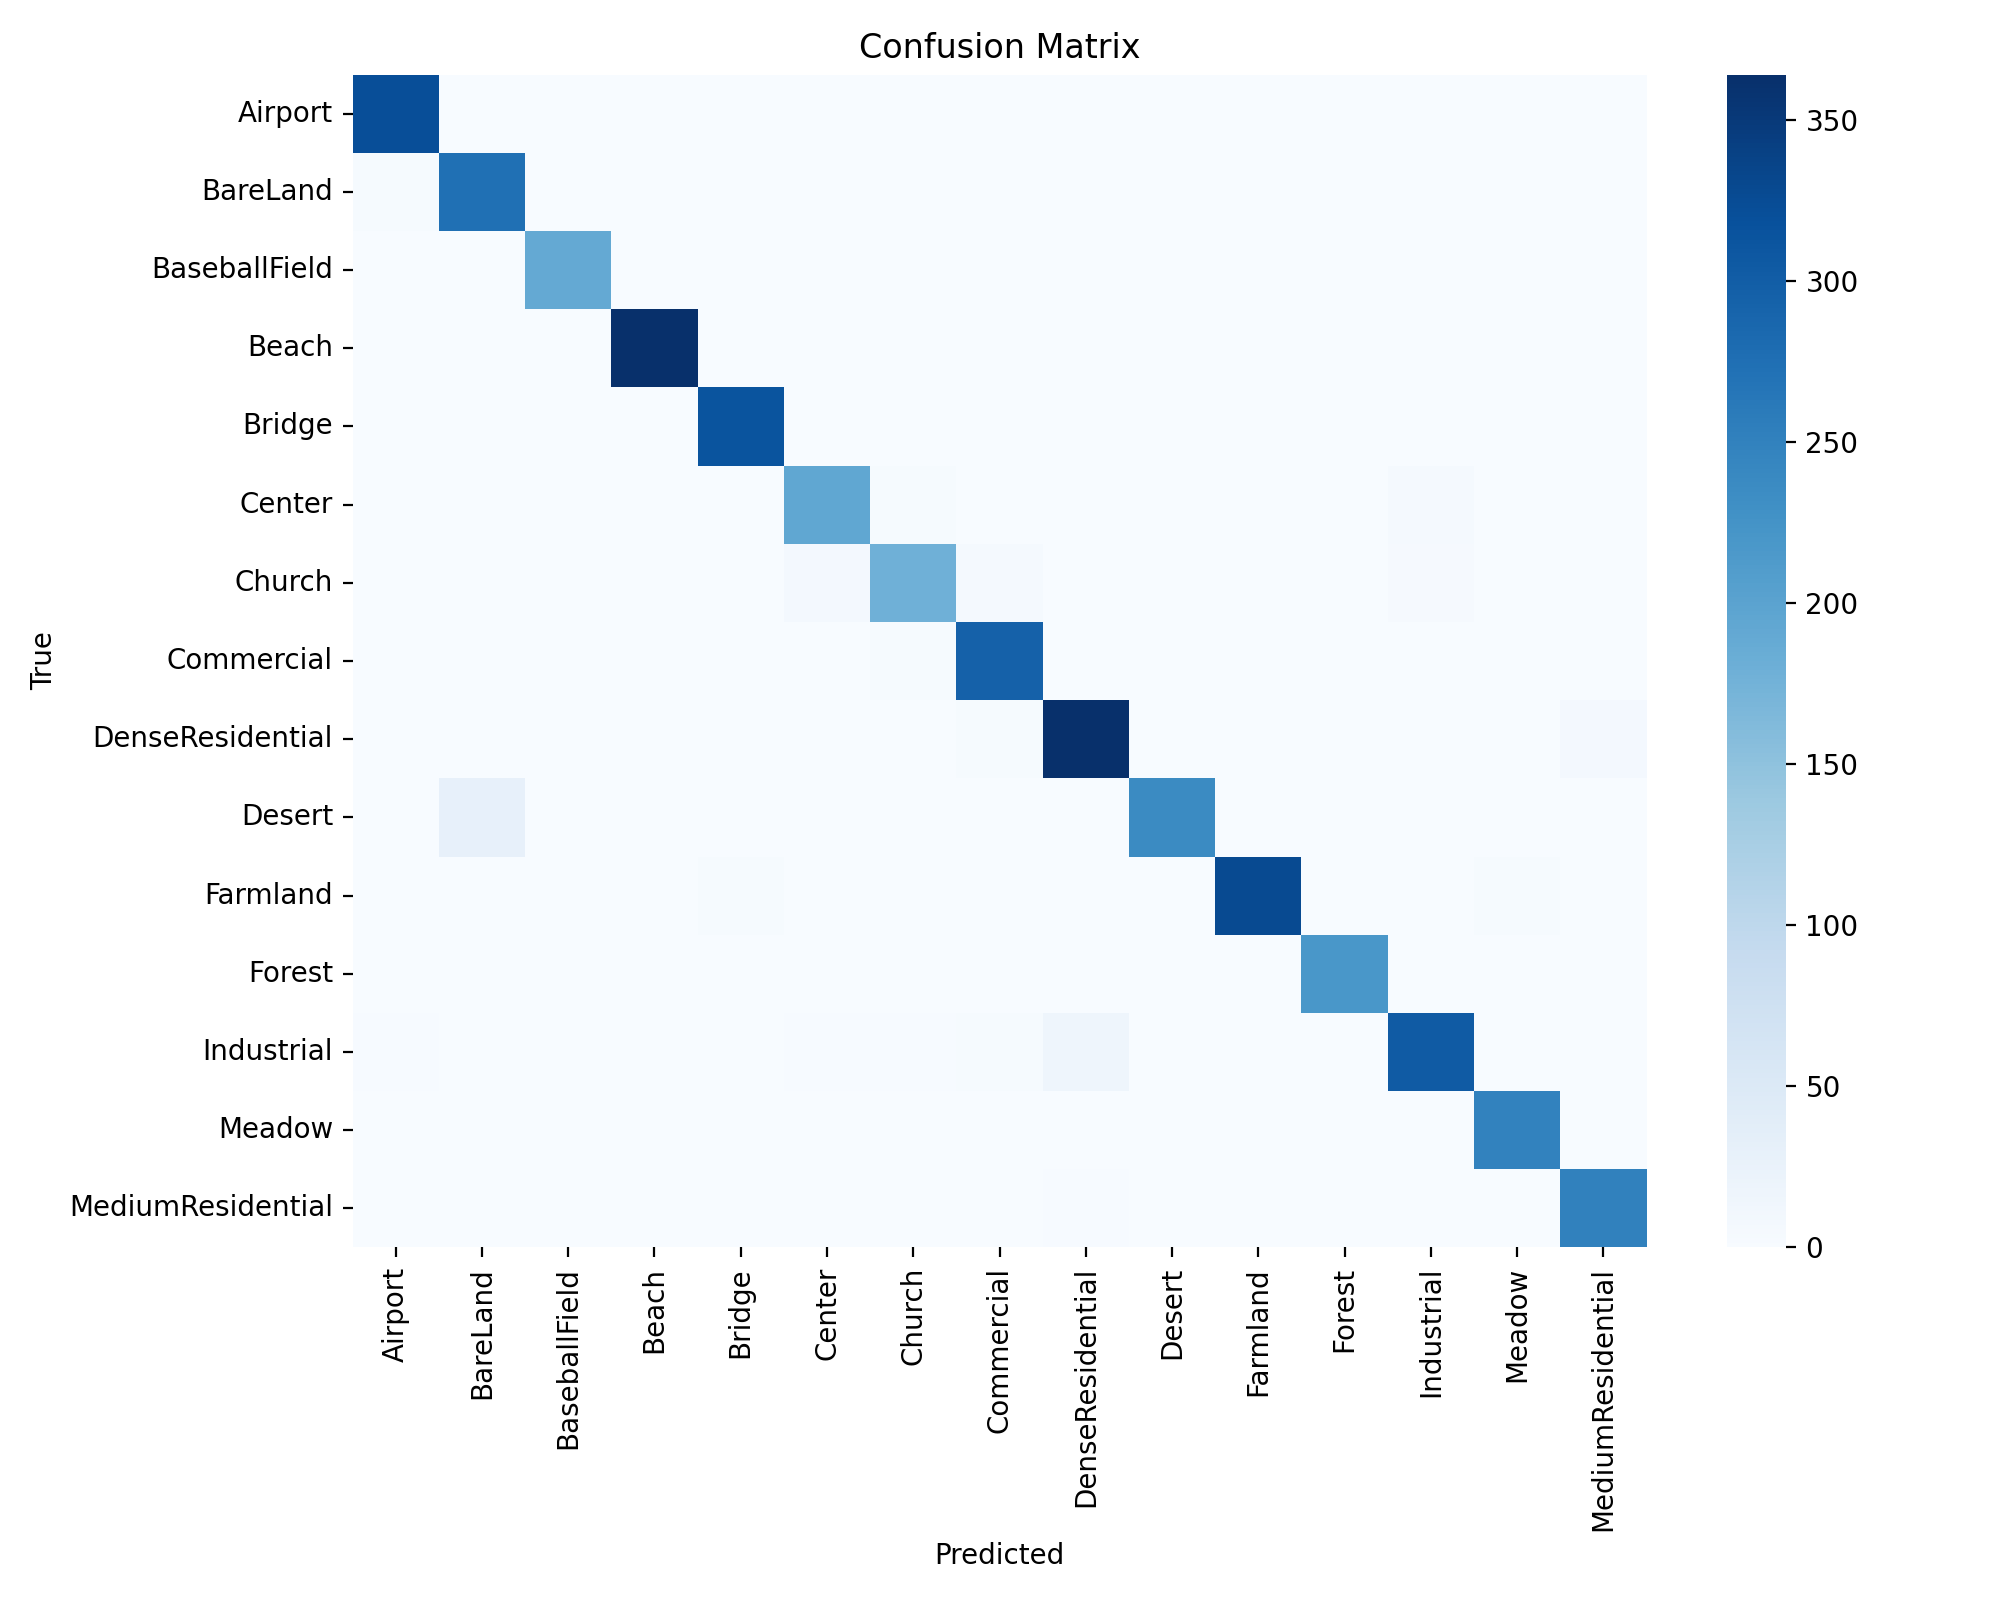
\includegraphics[width=\linewidth]{../../figures/aid_low20_baseline_confusion.png}
    \par\small (a) ConvNeXt-Tiny baseline
  \end{minipage}\hfill
  \begin{minipage}{0.48\linewidth}
    \centering
    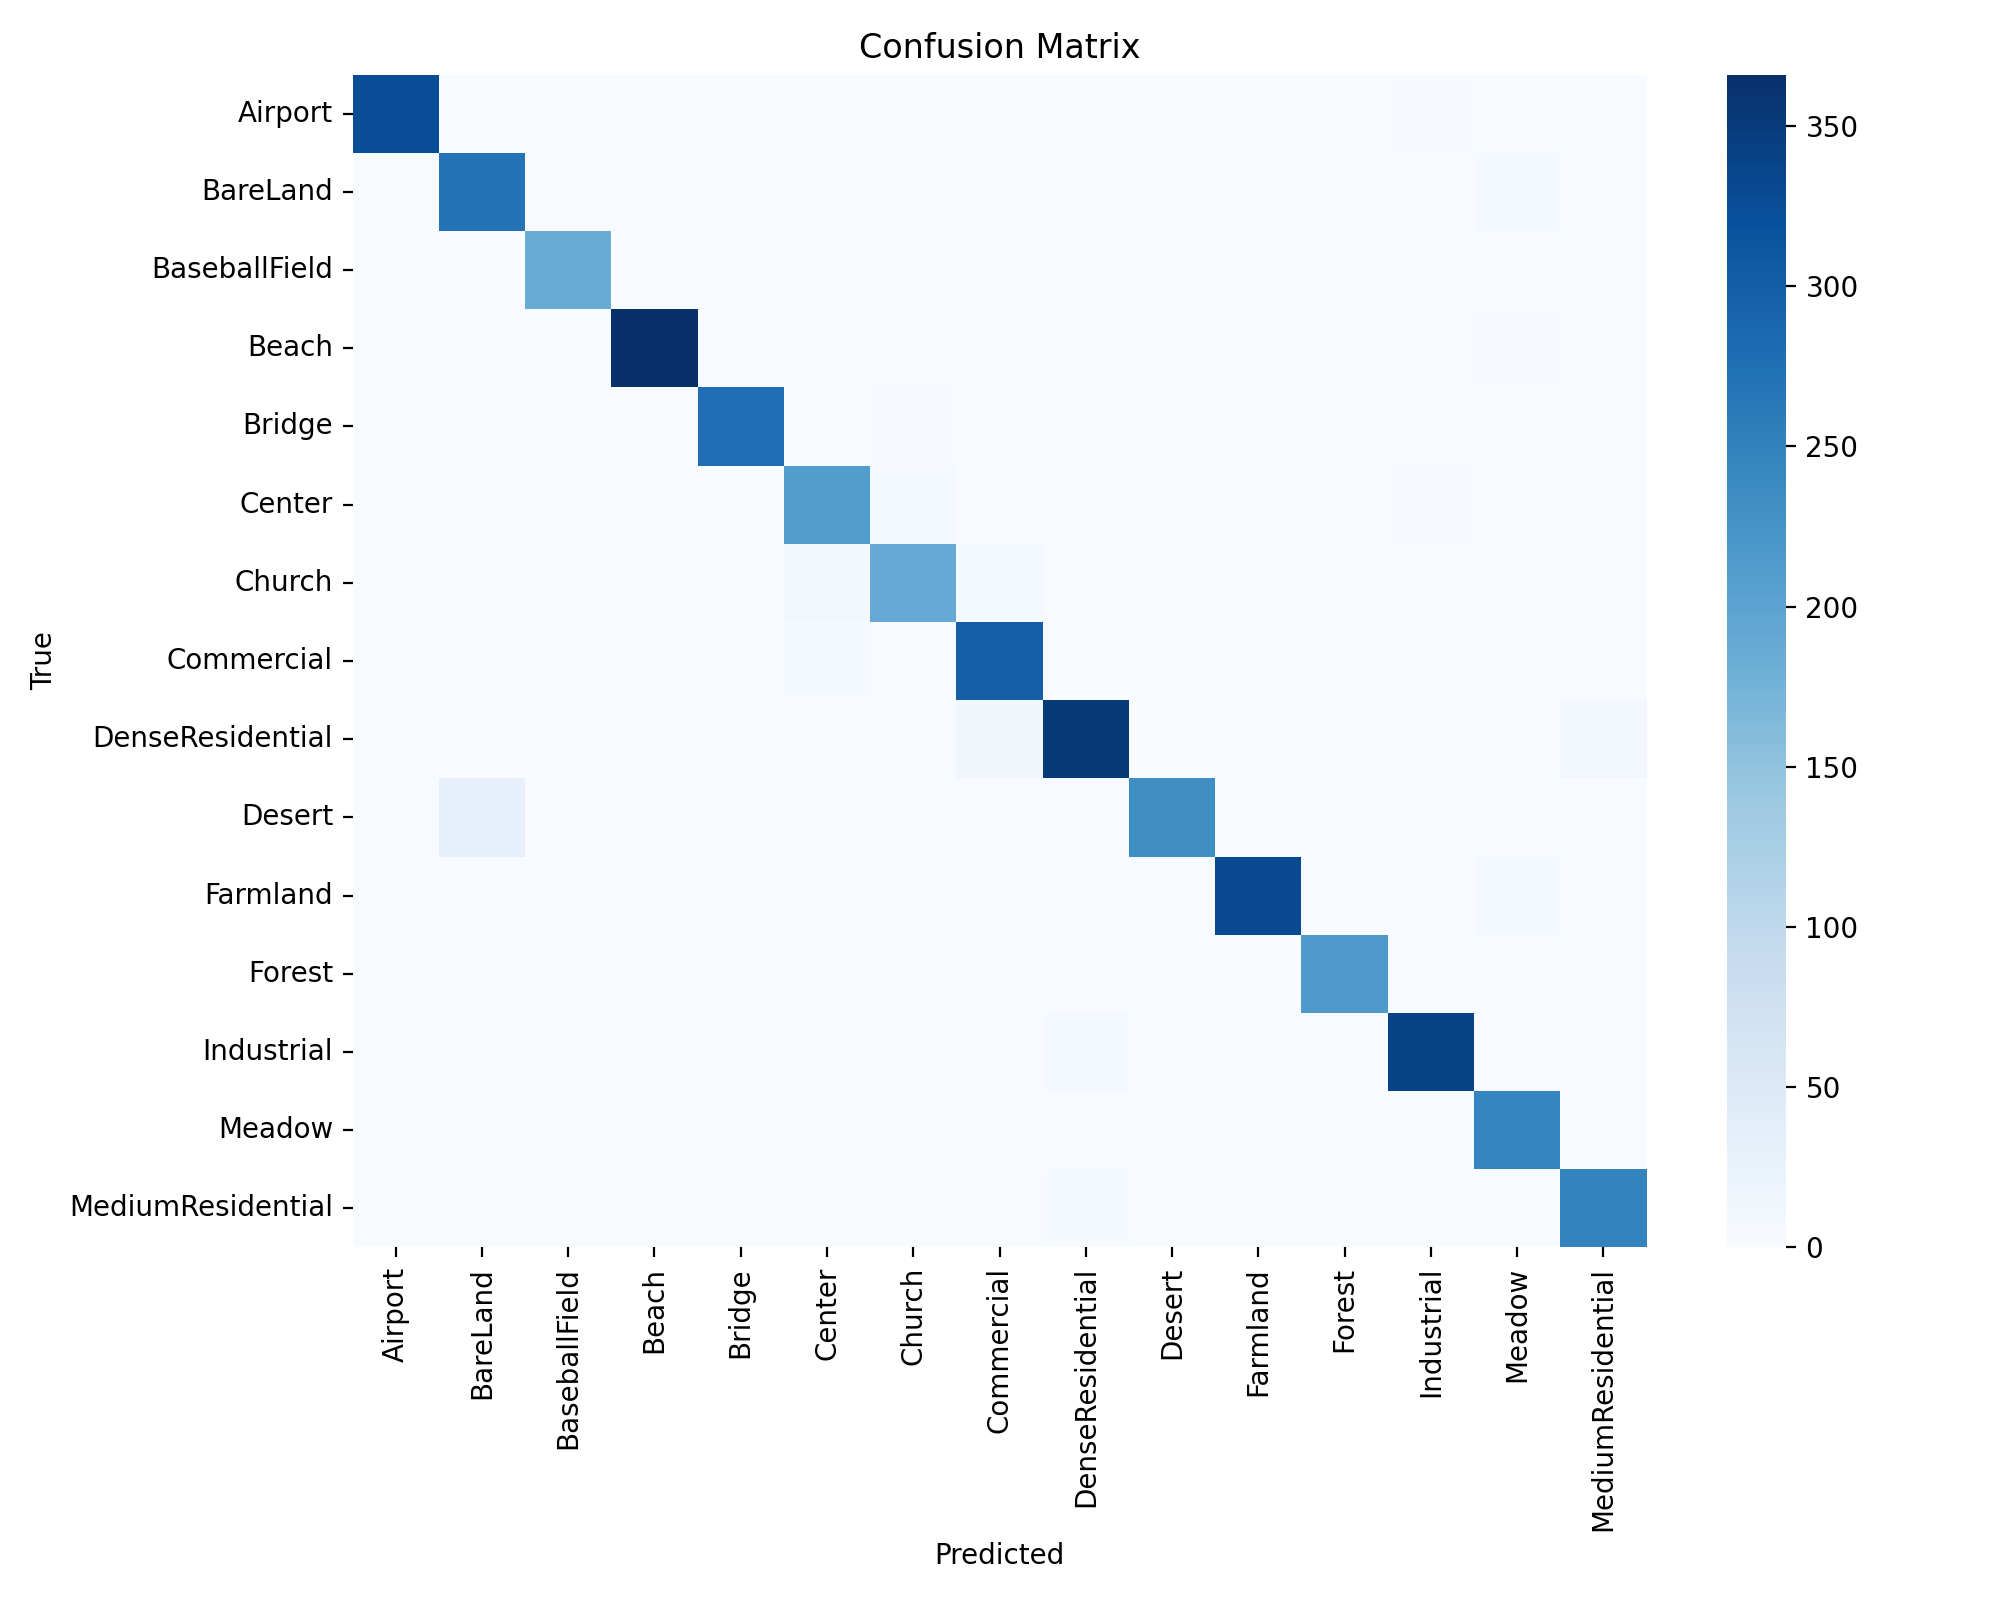
\includegraphics[width=\linewidth]{../../figures/aid_low20_full_confusion.png}
    \par\small (b) Proposed method
  \end{minipage}
  \caption{Confusion matrices on AID-low20 from seed 3407. Both subfigures use the same test partition, identical class ordering, and the same color scale.}
  \label{fig:aid_confusion}
\end{figure}

\begin{figure}
  \centering
  \begin{minipage}{0.48\linewidth}
    \centering
    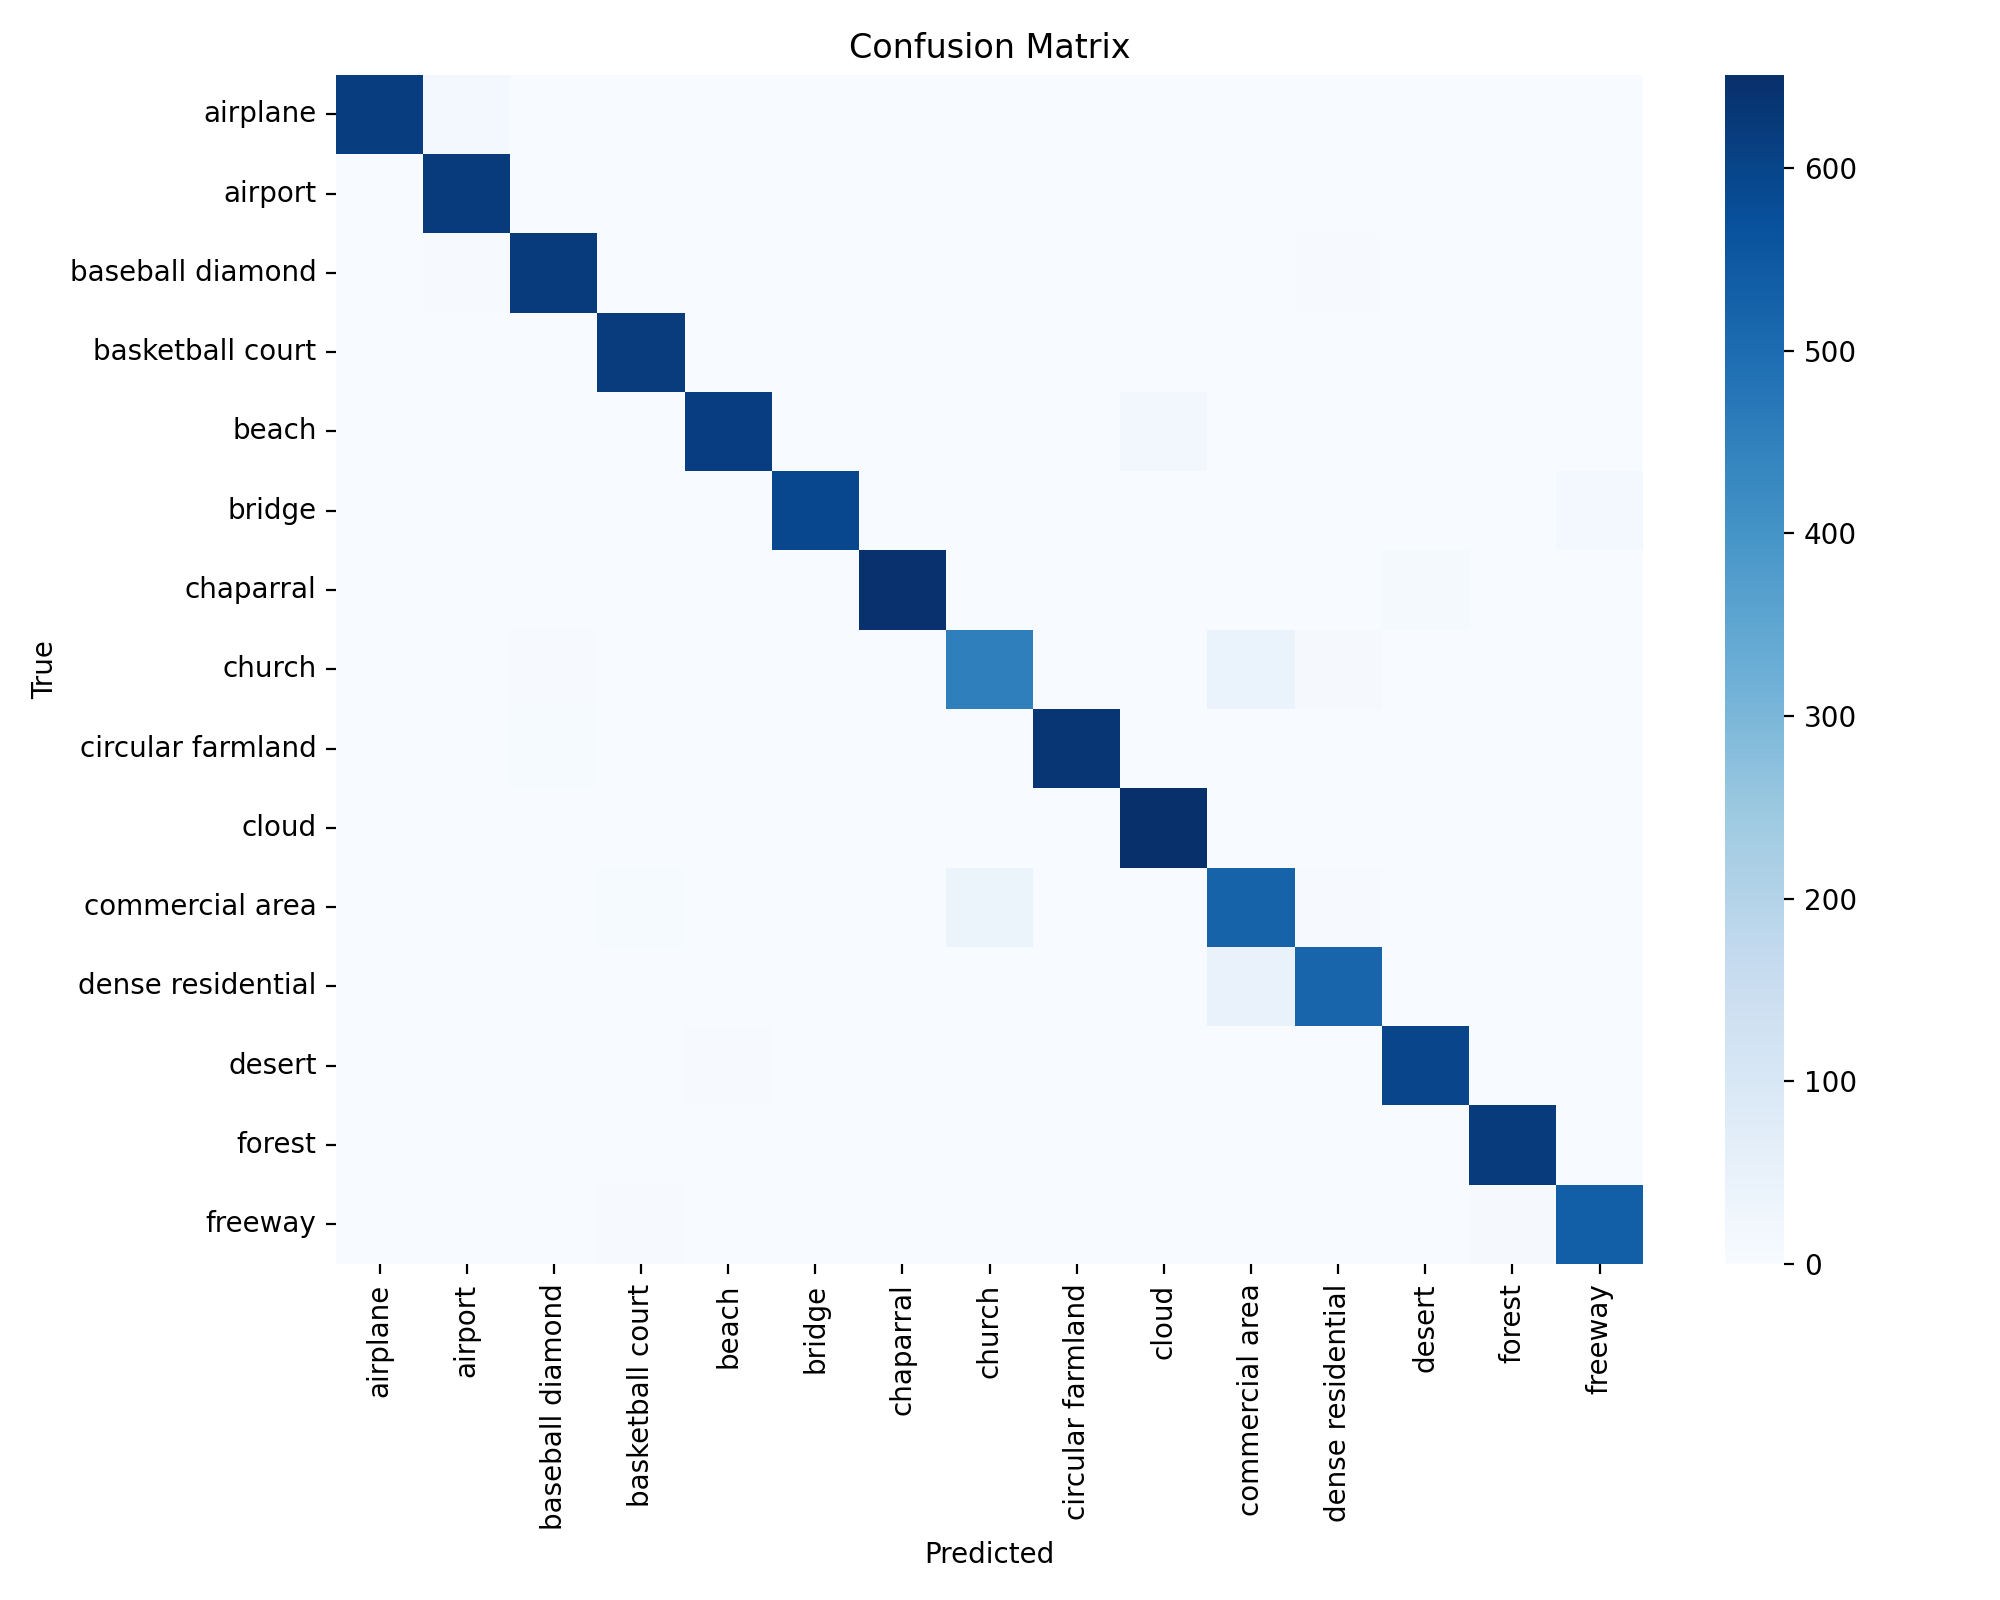
\includegraphics[width=\linewidth]{../../figures/nwpu_low20_baseline_confusion.png}
    \par\small (a) ConvNeXt-Tiny baseline
  \end{minipage}\hfill
  \begin{minipage}{0.48\linewidth}
    \centering
    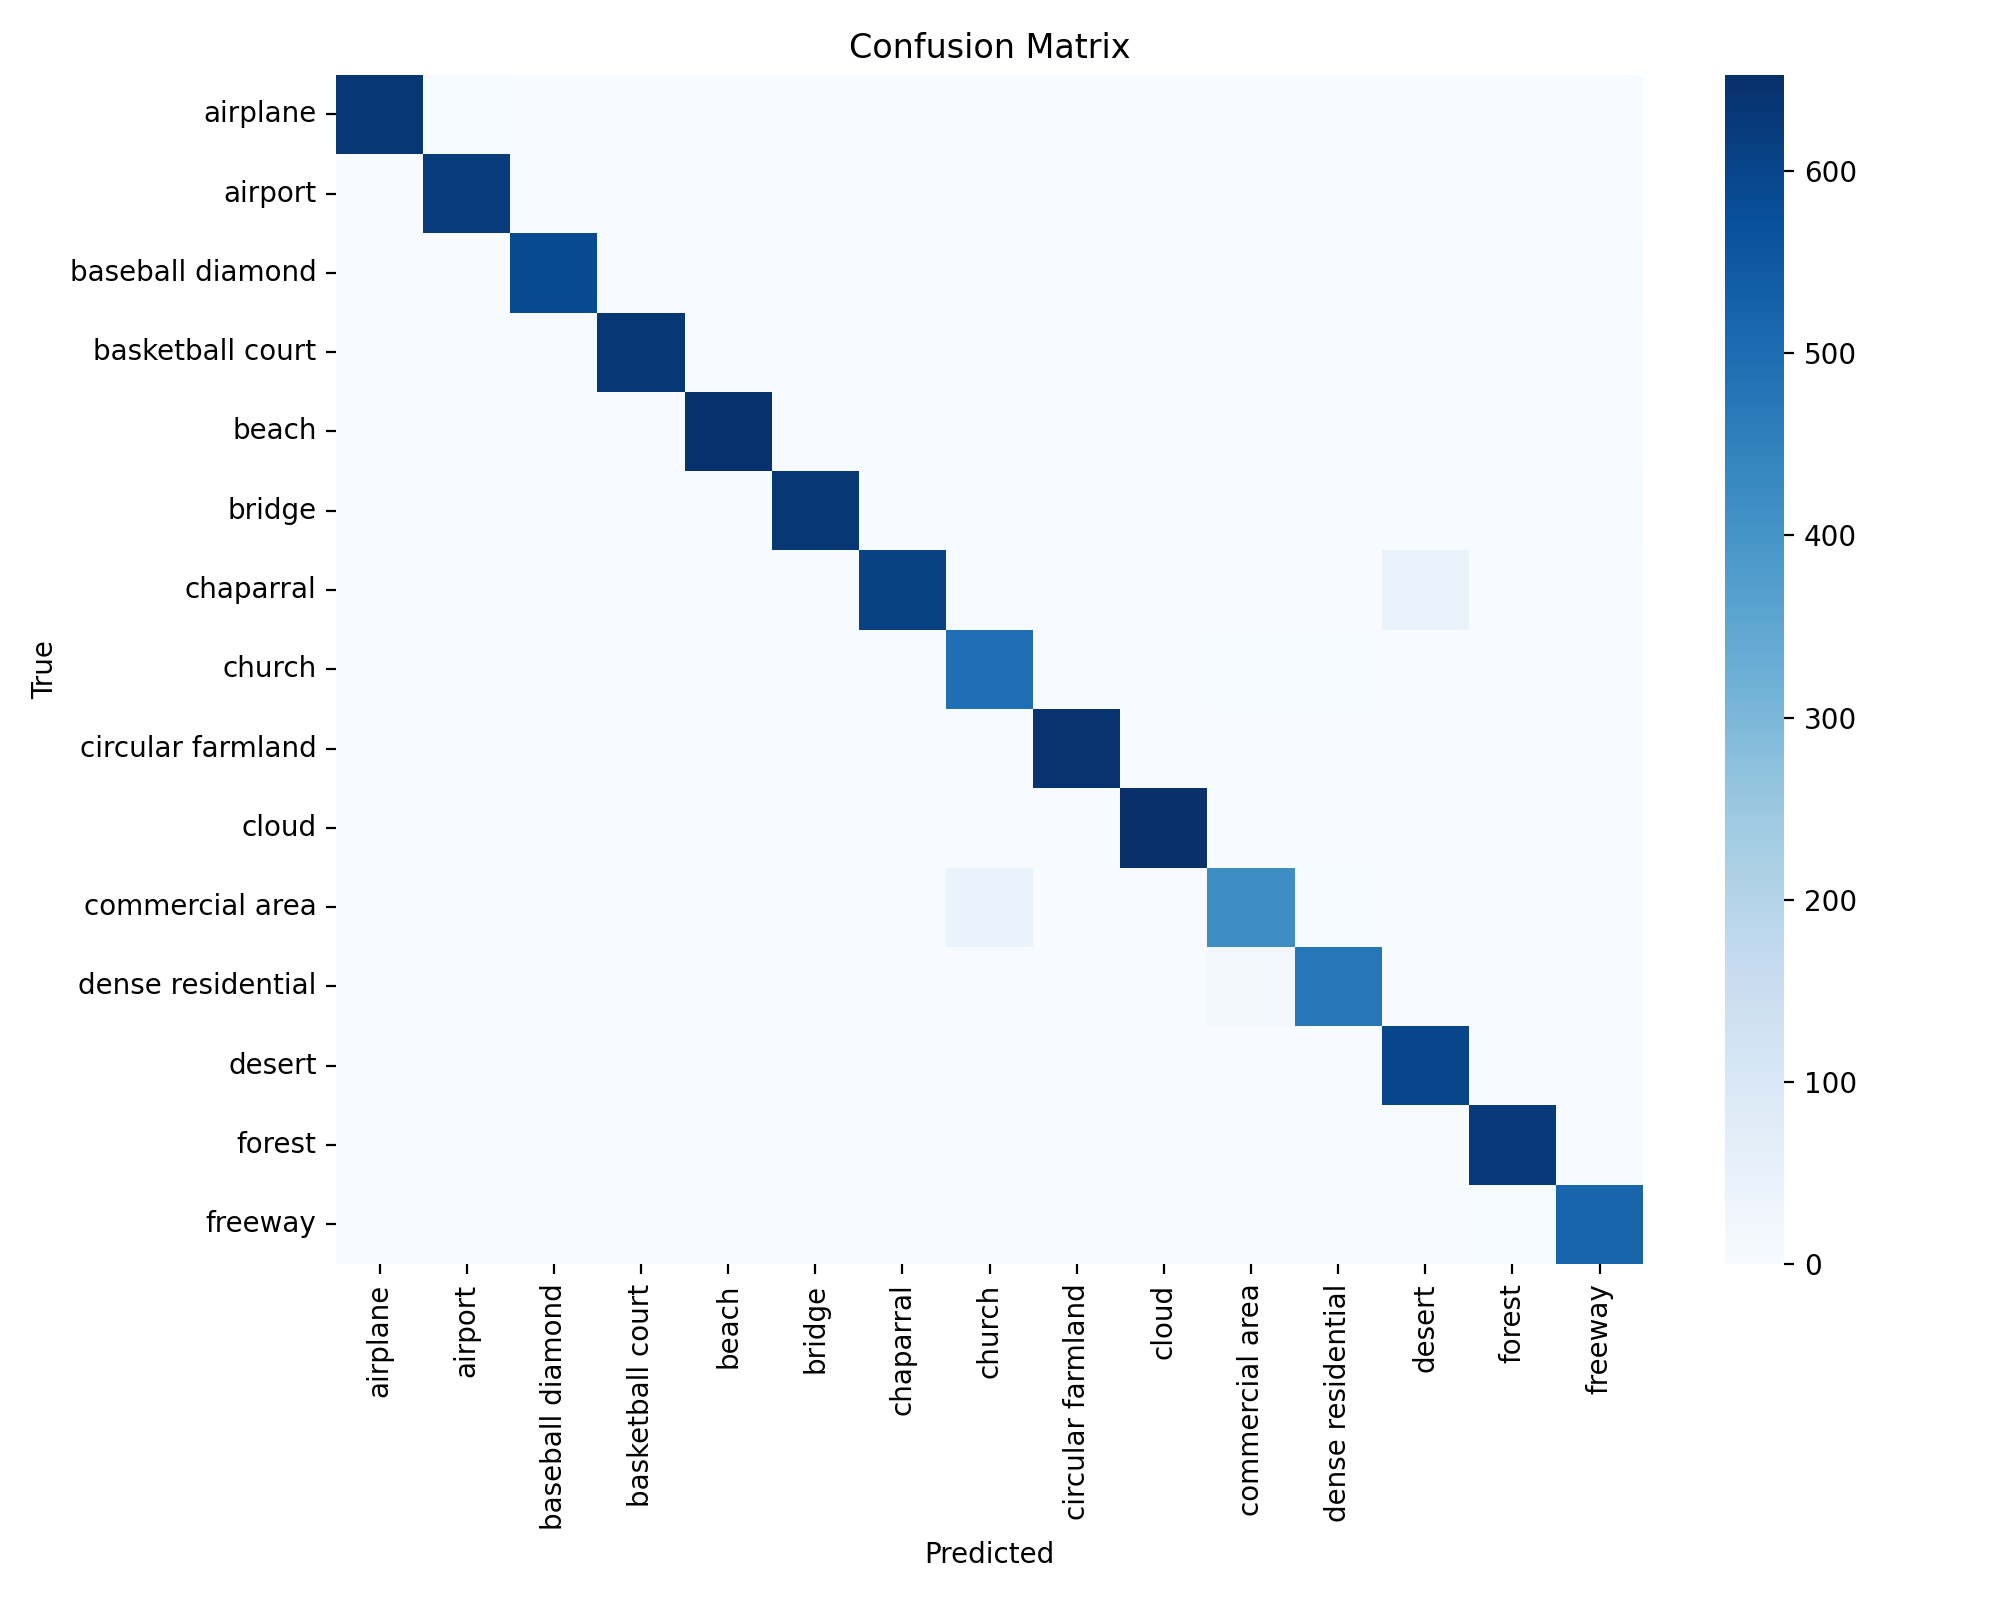
\includegraphics[width=\linewidth]{../../figures/nwpu_low20_full_confusion.png}
    \par\small (b) Proposed method
  \end{minipage}
  \caption{Confusion matrices on NWPU-low20 from seed 3407. Both subfigures use the same test partition, identical class ordering, and the same color scale.}
  \label{fig:nwpu_confusion}
\end{figure}

\subsection{Ablation Study}

We evaluate variants by removing one component at a time from the main DINOv2 setting. Tables~\ref{tab:aid-low20_ablation} and~\ref{tab:nwpu-low20_ablation} summarize the resulting three-seed ablations:
\begin{itemize}[leftmargin=1.5em]
  \item disabling partial finetuning (adapter-only) causes large degradation on both datasets;
  \item removing the adapter yields very similar mean OA on both datasets (AID: 0.9416 vs 0.9413, NWPU: 0.8793 vs 0.8790), but with larger seed variance than the full setting;
  \item removing feature-center regularization underperforms the full setting on both datasets in three-seed aggregation (AID: 0.9350 vs 0.9413, NWPU: 0.8722 vs 0.8790).
\end{itemize}
These results suggest that selective backbone finetuning contributes most of the mean improvement under the current protocol. The adapter mainly affects robustness and stability, whereas feature-center regularization shows a clear mean benefit on AID and a smaller positive shift on NWPU in three-seed aggregation. All key ablations are therefore reported with complete three-seed evidence. In particular, adapter-only drops to 0.8981 $\pm$ 0.0050 on AID and 0.7782 $\pm$ 0.0369 on NWPU, both below the full method (0.9413 and 0.8790, respectively), which supports keeping partial backbone finetuning in the final configuration under the current protocol. This same-backbone evidence also helps show that the final gains are not explained solely by switching from ConvNeXt to DINOv2; the controlled adaptation design within the DINOv2 route also contributes.

\begin{table}
  \centering
  \caption{Three-seed mean$\pm$std ablation results on AID-low20 under the fixed split protocol.}
  \label{tab:aid-low20_ablation}
  \begin{tabular}{l c c c}
    \toprule
    Variant & OA & AA & Kappa \\
    \midrule
    ConvNeXt-Tiny & 0.9179 $\pm$ 0.0086 & 0.9158 $\pm$ 0.0076 & 0.9150 $\pm$ 0.0089 \\
    NoCenter & 0.9350 $\pm$ 0.0075 & 0.9333 $\pm$ 0.0063 & 0.9327 $\pm$ 0.0078 \\
    NoAdapter & 0.9416 $\pm$ 0.0066 & 0.9391 $\pm$ 0.0067 & 0.9396 $\pm$ 0.0069 \\
    Adapter only & 0.8981 $\pm$ 0.0050 & 0.8969 $\pm$ 0.0044 & 0.8944 $\pm$ 0.0052 \\
    DINOv2-B (Adapter, FT) & 0.9413 $\pm$ 0.0036 & 0.9388 $\pm$ 0.0036 & 0.9392 $\pm$ 0.0037 \\
    \bottomrule
  \end{tabular}
\end{table}

\begin{table}
  \centering
  \caption{Three-seed mean$\pm$std ablation results on NWPU-low20 under the fixed split protocol.}
  \label{tab:nwpu-low20_ablation}
  \begin{tabular}{l c c c}
    \toprule
    Variant & OA & AA & Kappa \\
    \midrule
    ConvNeXt-Tiny & 0.8721 $\pm$ 0.0116 & 0.8721 $\pm$ 0.0116 & 0.8691 $\pm$ 0.0119 \\
    NoCenter & 0.8722 $\pm$ 0.0056 & 0.8722 $\pm$ 0.0056 & 0.8693 $\pm$ 0.0057 \\
    NoAdapter & 0.8793 $\pm$ 0.0112 & 0.8793 $\pm$ 0.0112 & 0.8765 $\pm$ 0.0115 \\
    Adapter only & 0.7782 $\pm$ 0.0369 & 0.7782 $\pm$ 0.0369 & 0.7731 $\pm$ 0.0378 \\
    DINOv2-B (Adapter, FT) & 0.8790 $\pm$ 0.0085 & 0.8790 $\pm$ 0.0085 & 0.8762 $\pm$ 0.0087 \\
    \bottomrule
  \end{tabular}
\end{table}


To make the component-role argument explicit, Table~\ref{tab:stability_results} compares the full method against the no-adapter and no-center variants. The no-adapter variant stays nearly tied in mean OA but shows larger variance on both datasets, which supports interpreting the adapter as a stability-oriented component rather than as the main source of mean improvement. The no-center variant is lower in mean OA on both datasets, with a larger gap on AID and a modest gap on NWPU, which supports retaining feature-center regularization in the final configuration.

\begin{table}
  \centering
  \scriptsize
  \setlength{\tabcolsep}{3pt}
  \caption{OA mean and standard deviation of the full method and the key same-backbone controls. NoAdapter isolates the role of the residual adapter, and NoCenter isolates the contribution of feature-center regularization.}
  \label{tab:stability_results}
  \begin{tabular}{l >{\raggedright\arraybackslash}p{0.22\textwidth} c c c}
    \toprule
    Dataset & Variant & OA Mean & OA Std & $\Delta$OA vs Full \\
    \midrule
    AID & NoAdapter & 0.9416 & 0.0066 & +0.0003 \\
    AID & NoCenter & 0.9350 & 0.0075 & -0.0063 \\
    AID & Full setting & 0.9413 & 0.0036 & +0.0000 \\
    NWPU & NoAdapter & 0.8793 & 0.0112 & +0.0003 \\
    NWPU & NoCenter & 0.8722 & 0.0056 & -0.0067 \\
    NWPU & Full setting & 0.8790 & 0.0085 & +0.0000 \\
    \bottomrule
  \end{tabular}
\end{table}


For additional transparency, Appendix Table~\ref{tab:seedwise_results} lists the per-seed OA values of the baseline, the full method, and the main ablation variants.

\subsection{Complexity Analysis}

Table~\ref{tab:complexity_results} reports the complexity tradeoff. The proposed route is not lightweight in total inference complexity, but it is parameter-efficient in terms of trainable subset and remains feasible on commodity 8GB GPUs. In practice, all final DINOv2 runs were trained on a single RTX 4060 Ti 8GB GPU using gradient checkpointing and gradient accumulation. This resource profile is important for computational geoscience settings where multi-GPU training may be unavailable but reproducible large-backbone transfer is still desirable. The no-adapter variant has almost identical FLOPs and slightly fewer trainable parameters, which further supports our interpretation that the adapter mainly contributes to optimization stability rather than raw model size reduction.

\begin{table}
  \centering
  \caption{Complexity comparison of the main baseline, the full method, and the no-adapter control. Trainable parameters are reported separately from total parameters.}
  \label{tab:complexity_results}
  \begin{tabular}{l c c c}
    \toprule
    Method & Total Params & Trainable Params & FLOPs \\
    \midrule
    ConvNeXt-Tiny & 27.8M & 27.8M & 8.93G \\
    DINOv2-B (NoAdapter, FT) & 86.6M & 7.12M & 43.93G \\
    DINOv2-B (Adapter, FT) & 87.0M & 7.51M & 43.93G \\
    \bottomrule
  \end{tabular}
\end{table}


\subsection{Visual Interpretation}

To keep the interpretation protocol consistent across convolutional and token-based backbones, we report gradient-based activation visualizations rather than strict layer-specific Grad-CAM for all models. Figures~\ref{fig:aid_activation} and~\ref{fig:nwpu_activation} show matched test examples from seed 3407. In these example pairs, the proposed method often places relatively more emphasis on class-defining structures and layout cues while showing less scattered background response than the ConvNeXt-Tiny baseline. This example-level qualitative tendency is clearer on AID, where the quantitative gain is also larger, and remains mild but generally aligned with the positive mean OA gain on NWPU. These activation maps are included only to contextualize model behavior under matched examples, not to establish superiority.

\begin{figure}
  \centering
  \begin{minipage}{0.48\linewidth}
    \centering
    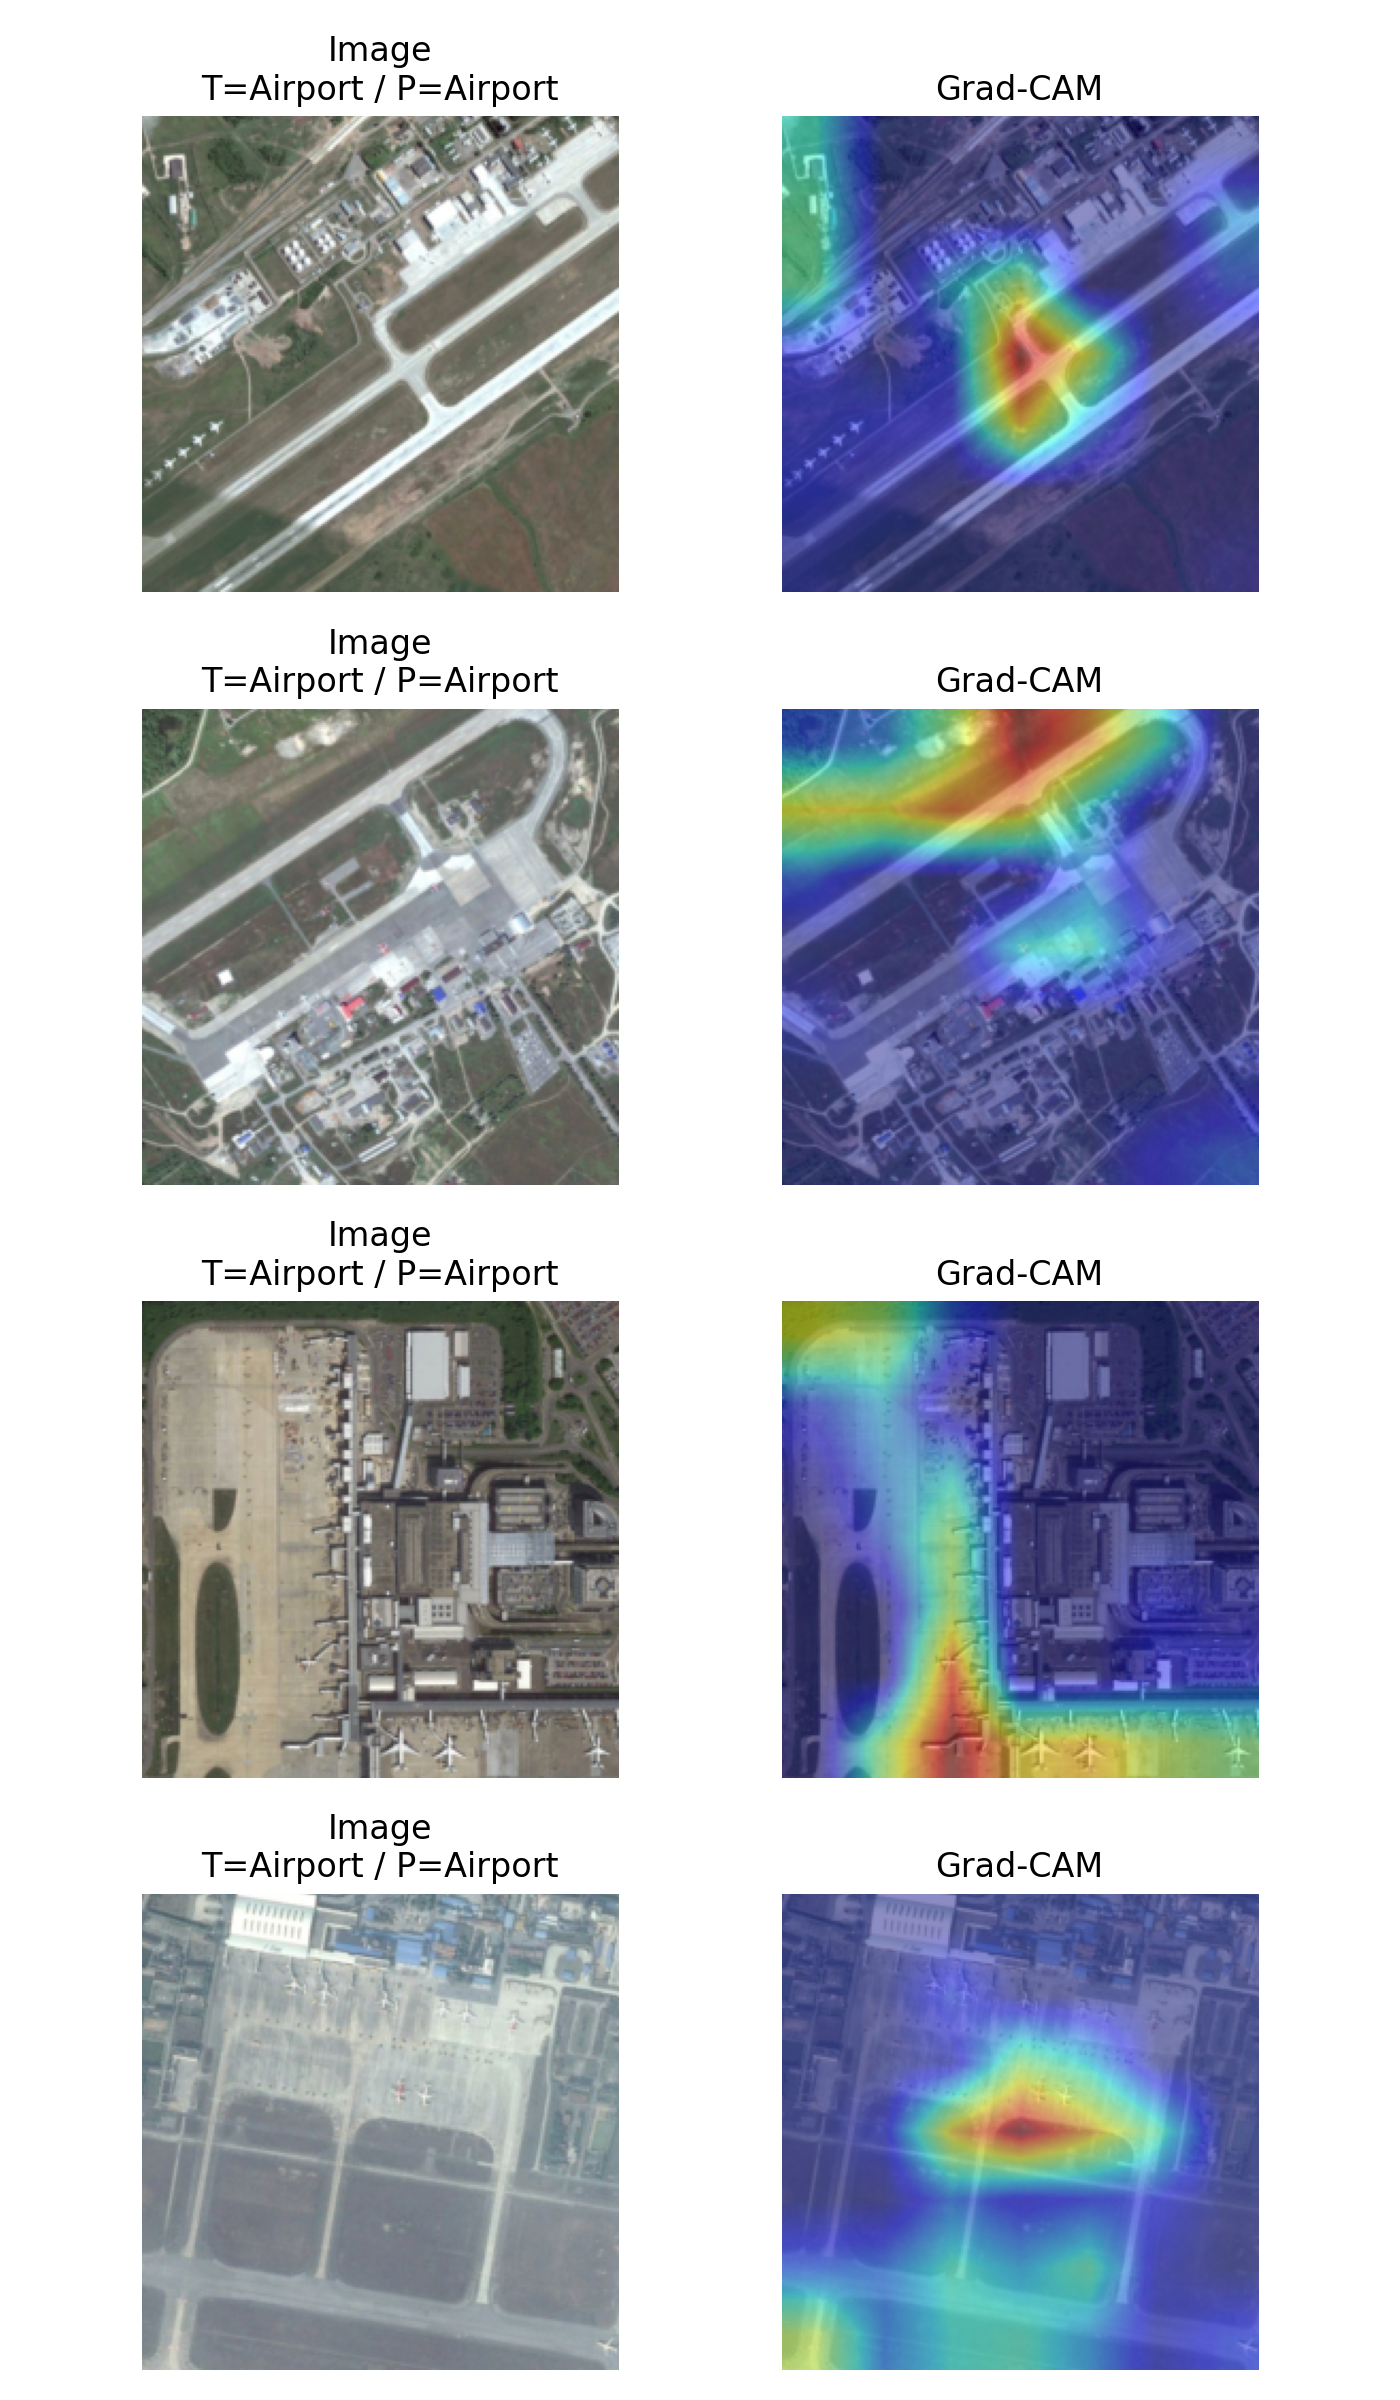
\includegraphics[width=\linewidth]{../../figures/aid_low20_baseline_activation.png}
    \par\small (a) ConvNeXt-Tiny baseline
  \end{minipage}\hfill
  \begin{minipage}{0.48\linewidth}
    \centering
    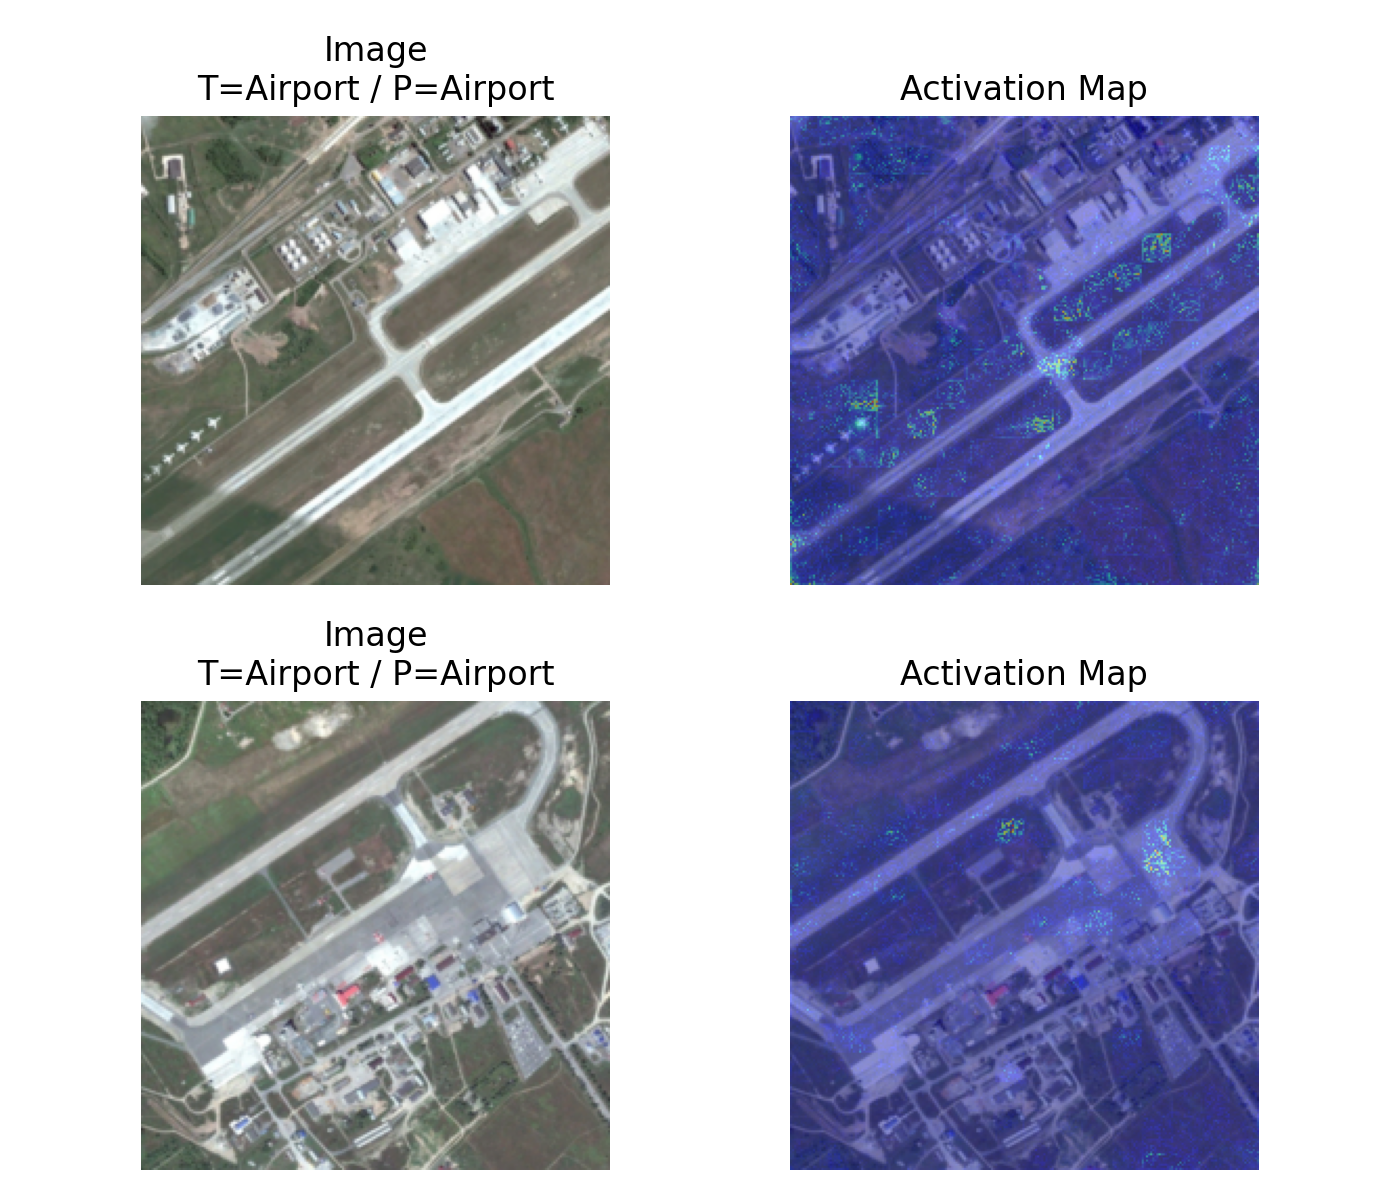
\includegraphics[width=\linewidth]{../../figures/aid_low20_full_activation.png}
    \par\small (b) Proposed method
  \end{minipage}
  \caption{Gradient-based activation visualizations on AID-low20 from seed 3407. Each pair uses the same test image and the same normalization pipeline for visual comparison.}
  \label{fig:aid_activation}
\end{figure}

\begin{figure}
  \centering
  \begin{minipage}{0.48\linewidth}
    \centering
    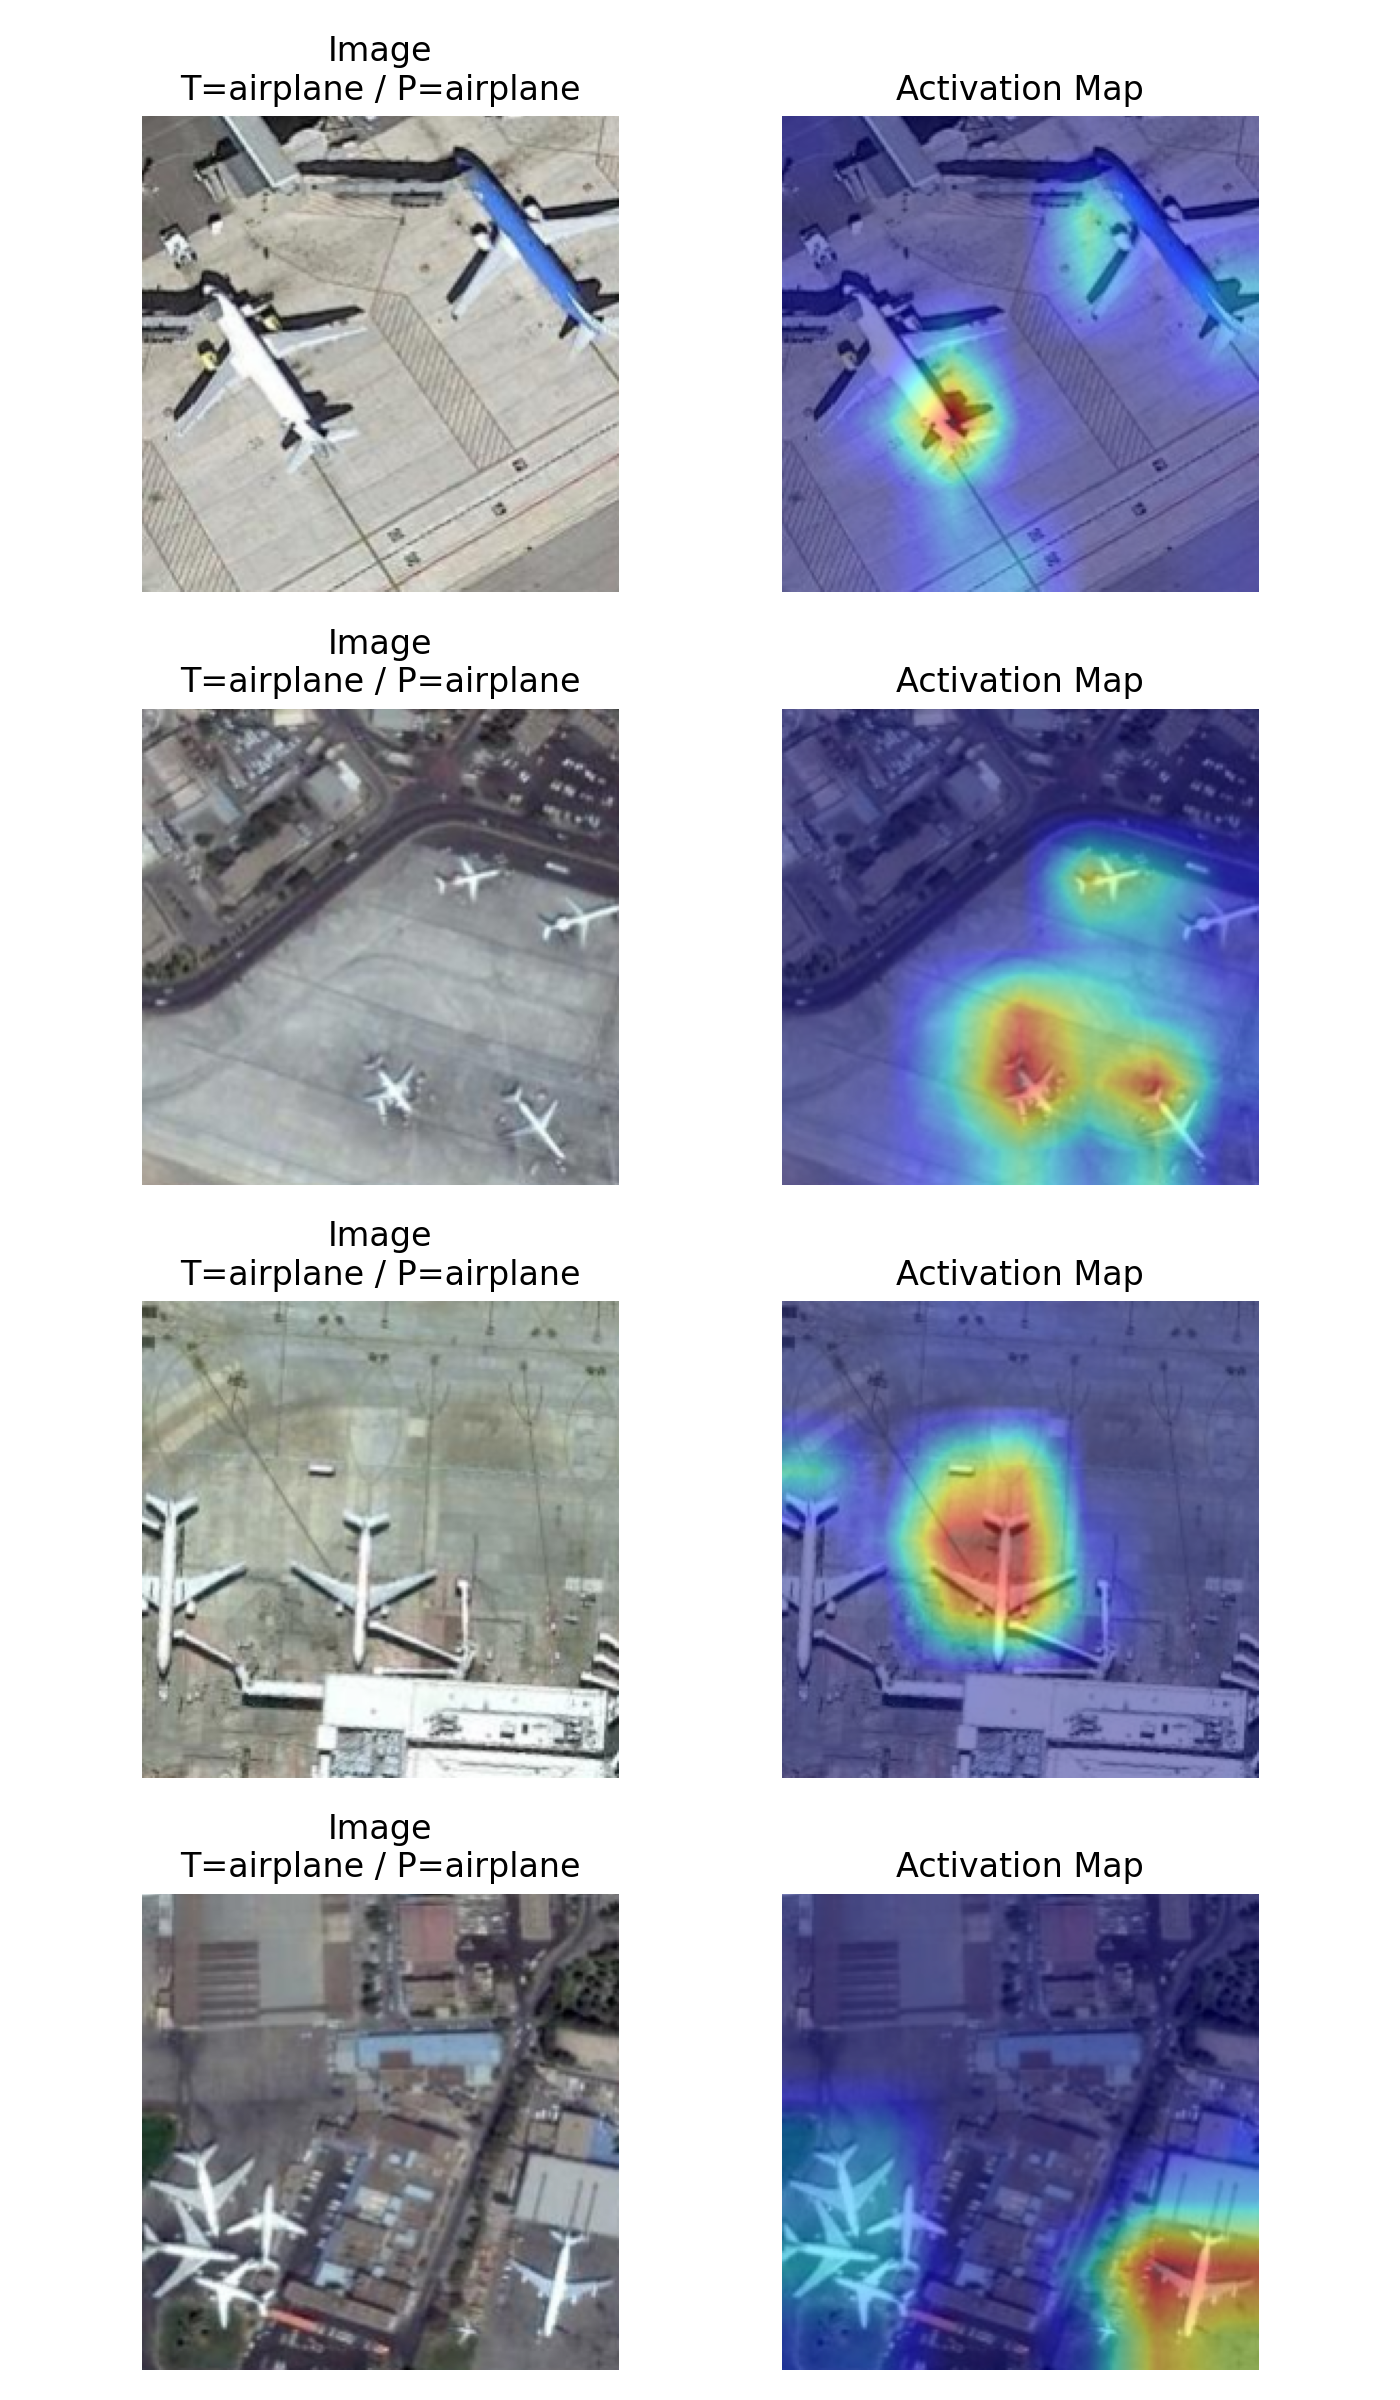
\includegraphics[width=\linewidth]{../../figures/nwpu_low20_baseline_activation.png}
    \par\small (a) ConvNeXt-Tiny baseline
  \end{minipage}\hfill
  \begin{minipage}{0.48\linewidth}
    \centering
    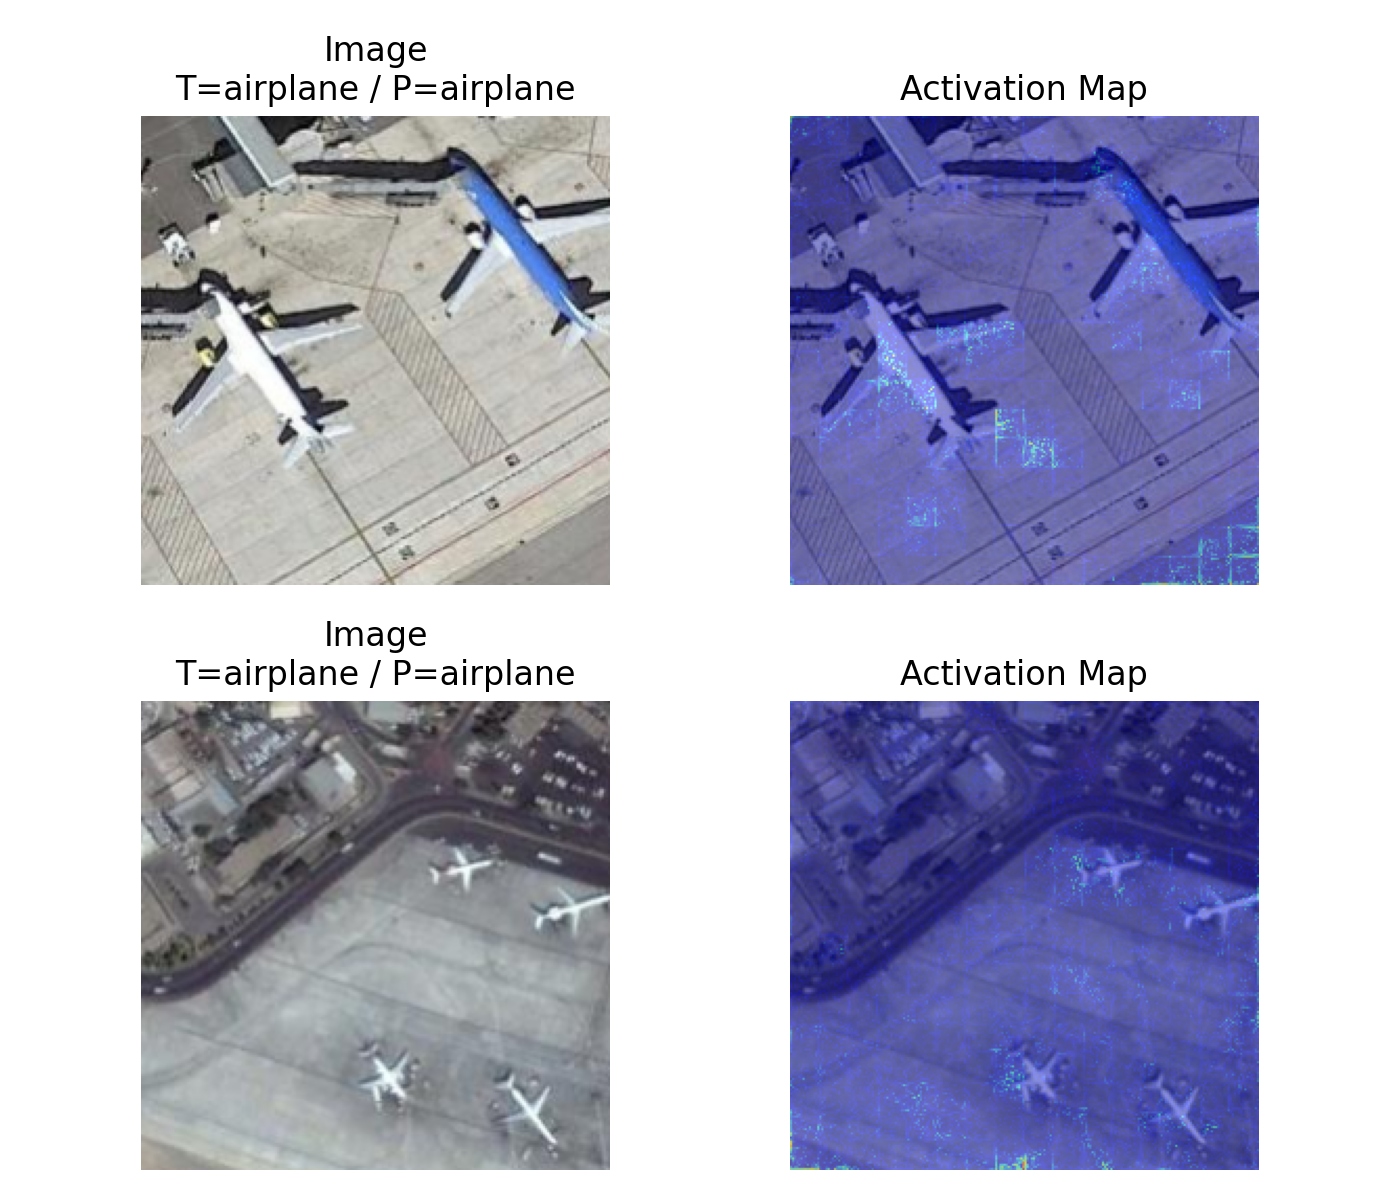
\includegraphics[width=\linewidth]{../../figures/nwpu_low20_full_activation.png}
    \par\small (b) Proposed method
  \end{minipage}
  \caption{Gradient-based activation visualizations on NWPU-low20 from seed 3407. Each pair uses the same test image and the same normalization pipeline for visual comparison.}
  \label{fig:nwpu_activation}
\end{figure}

\section{Conclusions}
\label{sec:conclusion}

This paper presents a reproducible selective-adaptation workflow for scarce-label remote sensing scene classification. Built on DINOv2-Base, the workflow combines selective finetuning, residual adapters, feature-center regularization, fixed split manifests, and scripted multi-seed reporting. Under the evaluated 20-shot protocol on AID and NWPU-RESISC45, it improves over a matched-split ConvNeXt-Tiny reference in three-seed mean overall accuracy while remaining trainable on a single 8 GB GPU. The main contribution is therefore a rebuildable geocomputing recipe for public-data low-shot evaluation, not a new remote-sensing-specific architecture.

The current evidence suggests that selective backbone finetuning is the main source of mean improvement, whereas the residual adapter mainly improves stability and the feature-center term mainly improves mean performance under the current protocol. The resulting contribution is therefore not a claim of lightweight inference or universal superiority, but a practical geocomputing recipe that can be rebuilt, audited, and extended on public data and modest hardware.

Several limitations remain. The gain on NWPU-RESISC45 is positive but modest, so the cross-dataset conclusion should be interpreted conservatively and read mainly as evidence that the workflow remains stable under a second public benchmark. The method is parameter-efficient in trainable subset rather than lightweight in total inference complexity. Finally, the current study covers two public datasets under a fixed 20-shot protocol; broader shot regimes and additional remote sensing domains would strengthen future validation. Even with these limits, the workflow provides a useful open baseline for scarce-label geospatial image analysis and a concrete starting point for follow-up geocomputing studies.

\section{Acknowledgments}
This work currently has no external funding to declare.

\newpage

\section*{Code availability}
Name of the code/library: Treatise scarce-label remote sensing classification workflow.

Contact: Chao Hou (2446099877@qq.com).

Hardware requirements: all final DINOv2 experiments were trained on a single NVIDIA RTX 4060 Ti 8 GB GPU with gradient checkpointing and gradient accumulation.

Program language: Python 3.11.

Software required: PyTorch environment defined by the project requirements file.

Program size: the release package contains source modules, experiment scripts, configuration files, and manuscript-build assets required to reproduce the reported workflow.

Redistributed assets exclude raw datasets and trained checkpoints.

The source code, experiment configurations, split-generation logic, aggregation scripts, and manuscript-table rebuild scripts are publicly available in the project GitHub repository.

Repository URL: \url{https://github.com/2446099877/paper_q2_cageo}.

Data availability: AID and NWPU-RESISC45 are public datasets cited in the manuscript. The repository provides split manifests and reproduction guidance, but does not redistribute raw images; users should obtain the original data from the official dataset sources under their respective terms.

A reviewer-safe archive containing the same source modules, manifests, configurations, and manuscript-build assets is retained for inspection convenience. The public repository is released under the MIT License.

\section{Seed-Wise OA Results}
\label{sec:appendix_seedwise}

For transparency, Table~\ref{tab:seedwise_results} reports the per-seed OA values of the baseline, the full method, and the key ablation variants that support the stability discussion in the main text. This appendix table is especially useful for checking whether a variant improves the mean through consistent gains or through a small number of favorable runs.

\begin{table}
  \centering
  \caption{Per-seed OA values on the fixed split manifests used by all compared methods.}
  \label{tab:seedwise_results}
  \begin{tabular}{l l c c c}
    \toprule
    Dataset & Variant & Seed 3407 & Seed 3408 & Seed 3409 \\
    \midrule
    AID-low20 & ConvNeXt-Tiny & 0.9232 & 0.9058 & 0.9248 \\
    AID-low20 & DINOv2-B (Adapter, FT) & 0.9365 & 0.9423 & 0.9452 \\
    AID-low20 & NoCenter & 0.9411 & 0.9395 & 0.9244 \\
    AID-low20 & NoAdapter & 0.9326 & 0.9438 & 0.9485 \\
    NWPU-low20 & ConvNeXt-Tiny & 0.8860 & 0.8726 & 0.8575 \\
    NWPU-low20 & DINOv2-B (Adapter, FT) & 0.8863 & 0.8835 & 0.8671 \\
    NWPU-low20 & NoCenter & 0.8768 & 0.8643 & 0.8755 \\
    NWPU-low20 & NoAdapter & 0.8946 & 0.8753 & 0.8680 \\
    \bottomrule
  \end{tabular}
\end{table}


\section{Reproducibility Notes}
\label{sec:appendix_reproducibility}

All compared methods use seed-controlled manifests generated by class-wise shuffling under the same split rule: 20 training images and 10 validation images per class, with all remaining images used for testing. For a fixed seed, the same manifest is reused by every compared method, so the ConvNeXt baseline and all DINOv2 variants are evaluated on identical data partitions. The public repository already includes the split-generation logic, model definitions, training loop, multi-seed aggregation utilities, and the scripts used to rebuild the manuscript tables.

The final DINOv2 setting uses the configuration corresponding to the 20-shot protocol, partial finetuning of the last transformer block, adapter bottleneck dimension 256, and feature-center loss weight 0.02. The final ConvNeXt baseline uses the same seed protocol and early-stopping logic but a lighter backbone and larger batch size. No seed-specific hyperparameter changes are introduced after the protocol is fixed. The accompanying reproducibility package also retains the manuscript build script and the submission-readiness checker used to regenerate the final C\&G submission PDF.

\bibliographystyle{cas-model2-names}
\bibliography{../../references}

\end{document}
